\documentclass{article}
\usepackage{tikz}
\usetikzlibrary{arrows.meta,arrows}
\begin{document}
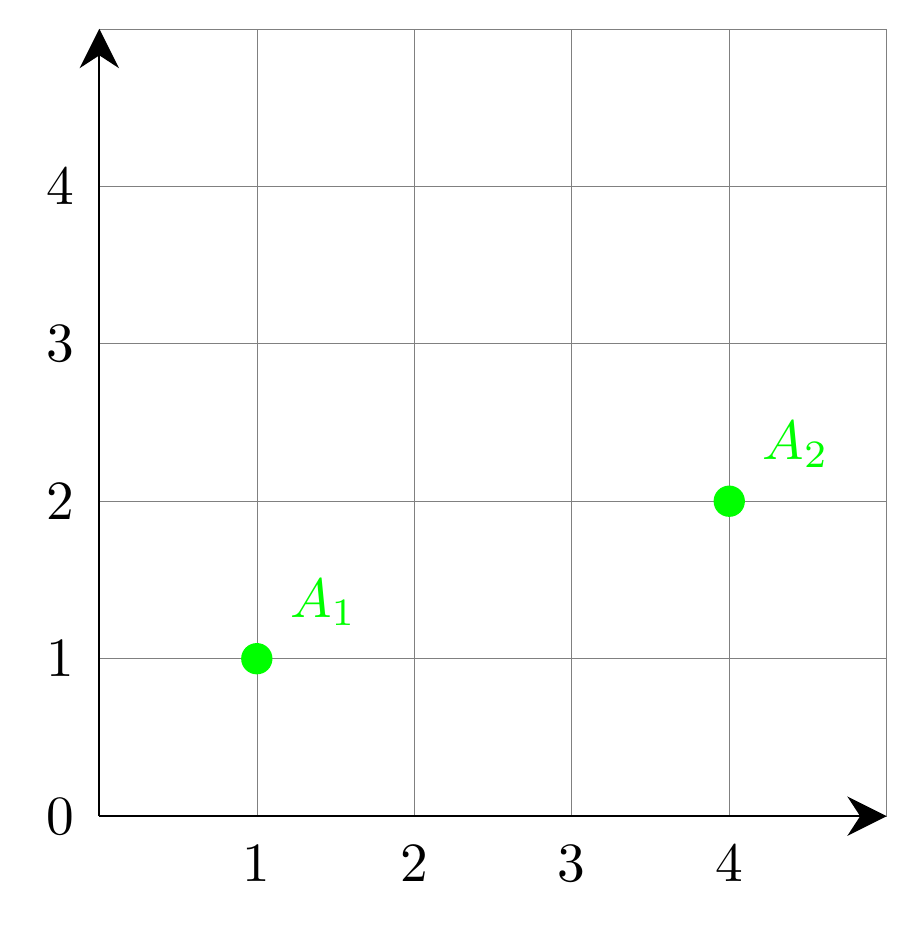
\begin{tikzpicture}[thick,scale=1, every node/.style={scale=2}]

% draw grid
\draw[step=2cm,gray,very thin] (0,0)grid(10,10);

% draw axes
\draw [-{Stealth[length=5mm, width=5mm]}](0,0) -- (10,0);
\draw [-{Stealth[length=5mm, width=5mm]}](0,0) -- (0,10);

% add axes labels
\node[fill=white,minimum height=10] at (-0.5,0){0};
\node[fill=white,minimum height=10] at (-0.5,2){1};
\node[fill=white,minimum height=10] at (-0.5,4){2};
\node[fill=white,minimum height=10] at (-0.5,6){3};
\node[fill=white,minimum height=10] at (-0.5,8){4};
\node[fill=white,minimum height=10] at (2,-0.6){1};
\node[fill=white,minimum height=10] at (4,-0.6){2};
\node[fill=white,minimum height=10] at (6,-0.6){3};
\node[fill=white,minimum height=10] at (8,-0.6){4};

% add points
\node[circle, fill=green,inner sep=2pt,label=45:\color{green}$A_1$]at (2,2){};
\node[circle, fill=green,inner sep=2pt,label=45:\color{green}$A_2$]at (8,4){};

\end{tikzpicture}
\end{document}
